\chapter{gaNitada oMdu taMtarx}


BAsakxrf avara maDadi kamala avaroMdige suKavAda jiVvana naDesutitxdadxru. mudAdxda eraDu makakxLu AratigoMdu kiVtiRgoMdu eMbaMte. modalneya maga sureVshf avanige hatutx vaSaR. eraDaneyavaLu magaLu perxVma. avaLige aidu vaSaR. parxtiyoMdu vaSaRvU ibabxru makakxLalilx yArAdarobabxra huTuTx hababxda dina oMdu kAyaRkarxma EpaRDisutitxdadxru. oMdoMdu vaSaR oMdoMdu riVtiya ATa, akakxpakakxda mane makakxLu, saMbaMdhikara makakxLanunx A kAyaRkarxmakekx AhAvxnisutitxdadxru. A sala tamamx maneya ibabxru makakxLu seVri hanonxMdu jana makakxLidadxru. BAsakxrf avara tamamx shaMkarf gaNitada mAsatxru. balu budidhxvaMtaru. avatutx makakxLige ADisuva ATadalilx aNaNxna makakxLibabxrigU bahumAna baruvaMte budidhx upayoVgisi oMdu ATa AraMBisidaru.

hanonxMdu makakxLanunx vaqtAtxkAradalilx nililxsidaru. aNaNxna ibabxru makakxLanunx eraDaneya matutx ELaneya sAthxnadalilx nililxsidaru. ATada niyama hiVgitutx. oMdariMda AraMBisi, mUraneya sAthxnadalilxruvavaru vaqtatxdiMda horage hoVgabeVku. kaDeyalilx uLiyuva ibabxru gedadxMte sari I riVti vaqtAtxkAravAgi nililxsidaru.
\begin{figure}[H]
\centering
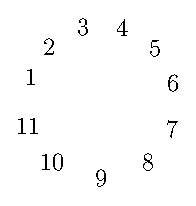
\includegraphics{src/figures/fig1.eps}
\end{figure}

oMdariMda AraMBisi, mUraneyavaru vaqtatxdiMda horage hoVgabeVku. adaraMte modalaneya sutitxnalilx $3$, $6$, $9$ sAthxnadalilxruvavaru vaqtatxdiMda horagaDe hoVdaru.
\begin{figure}[H]
\centering
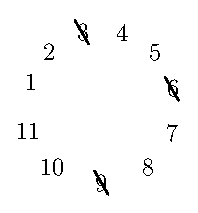
\includegraphics{src/figures/fig2.eps}
\end{figure}

uLidavaranunx punaH vaqtAtxkAradalilx nililxsidaru. horagaDe hoVdare kone saMKeyxyiMda AraMBisi aMdare $10$ riMda AraMBisi mUraneyavaru vaqtatxdiMda horakekx hoVgabeVku. eraDaneya sutitxnalilx $1$, $5$, $10$ ra sAthxnadalilxruvavaru vaqtatxda horagaDe uLidaru.
\begin{figure}[H]
\centering
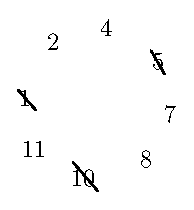
\includegraphics{src/figures/fig3.eps}
\end{figure}

uLidavaranunx punaH vaqtAtxkAradalilx nililxsidaru. $11$ riMda AraMBisi mUraneyavaru vaqtatxdiMda horage hoVgabeVku. I mUraneya sutitxnalilx horage hoVdavaru $4$ matutx $11$ neya sAthxnadalilxdadxvaru. 
\begin{figure}[H]
\centering
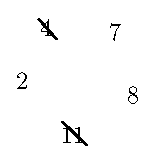
\includegraphics{src/figures/fig4.eps}
\end{figure}

uLida mUru makakxLanunx punaH vaqtAtxkAradalelxV nililxsidaru. $2$ riMda AraMBisi mUraneyavaru vaqtatxdiMda horakekx hoVgabeVku. I kaDe nAlakxneya sutitxnalilx $8$ neya sAthxnadalilxdadxvaru vaqtatxdiMda horakekx hoVdaru.
\begin{figure}[H]
\centering
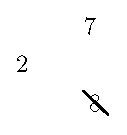
\includegraphics{src/figures/fig5.eps}
\end{figure}

koneyalilx uLidavaru $2$ matutx $7$ neya sAthxnadalilxdadx BAsakxrf avara makakxLu. aMtU shaMkarf avara budidhxvaMtike matAyxrigU tiLidiralilalx. avarobabxrige gotitxtutx. keVvala budidhx idadxre sAladu. kelavu sala tatatxvX gotitxrabeVku. idanenxV vijAcnxnadalilx, nAvu veYjAcnxnikaparxjecnx enunxvudu. 
